% Gemini theme
% https://github.com/anishathalye/gemini

\documentclass[final,20pt]{beamer}

% ====================
% Packages
% ====================

\usepackage[ngerman]{babel}
\usepackage[T1]{fontenc}
\usepackage{lmodern}
\usepackage[size=a1,orientation=portrait,scale=1.2]{beamerposter}
\usetheme{gemini}
\usecolortheme{gemini}
\usepackage{graphicx}
\usepackage{tikz}
\usepackage{pgfplots}
\usepackage{svg}

% ====================
% Lengths
% ====================

% If you have N columns, choose \sepwidth and \colwidth such that
% (N+1)*\sepwidth + N*\colwidth = \paperwidth
\newlength{\sepwidth}
\newlength{\colwidth}
\setlength{\sepwidth}{0.02\paperwidth}
\setlength{\colwidth}{0.47\paperwidth}

\newcommand{\separatorcolumn}{\begin{column}{\sepwidth}\end{column}}
\addto\extrasngerman{\def\figureautorefname{Abb.}}
% ====================
% Title
% ====================

\title{Apoplexy - Ein Fitnesstracker zur Rehabilitation von Schlaganfall-Patienten?}

\author{Lukas Rost}
\institute{Albert-Schweitzer-Gymnasium Erfurt}

% ====================
% Body
% ====================

\begin{document}

\begin{frame}[t]
\begin{columns}[t]
\separatorcolumn

\begin{column}{\colwidth}

  \begin{alertblock}{Schlaganfall als Krankheitsbild}
  	\begin{itemize}
  		\item plötzliche Durchblutungsstörung im Gehirn
  		\item regionaler Mangel an Sauerstoff und Nährstoffen
  		\item Absterben von Gehirngewebe
  		\item zwei Arten:
  		\begin{enumerate}
  			\item ischämischer Infarkt (mangelnde Durchblutung) aufgrund von Gefäßverschlüssen
  			\item hämorrhagischer Infarkt (Hirnblutungen) aufgrund von geplatzten Blutgefäßen
  		\end{enumerate}
  		\item \textbf{Vorbote:} transistorisch-ischämische Attacken (vorübergehende neurologische Ausfälle)
  		\item \textbf{Symptome:}
  		\begin{itemize}
  			\item halbseitige Körperlähmung
  			\item Sprachstörungen und eingeschränktes Sprachverständnis
  			\item Sehstörungen, Gleichgewichtsprobleme und Verwirrtheit
  		\end{itemize}
  		\item \textbf{Erkennung} durch den FAST-Test (Cincinnati Prehospital Stroke Scale):
  		\begin{enumerate}
  			\item \textbf{Face:} Person kann nur mit einer Gesichtshälfte lächeln
  			\item \textbf{Arms:} Unfähigkeit, beide Arme mit nach oben geöffneten Handflächen nach vorne
  			zu strecken
  			\item \textbf{Speech:} undeutliche Aussprache
  			\item \textbf{Time:} umgehende Verständigung des Rettungsdienstes
  		\end{enumerate}
  		\item \textbf{Risikofaktoren:}
  		 \begin{itemize}
  		 	\item Bluthochdruck und Rauchen
  		 	\item Diabetes, Übergewicht und Bewegungsmangel
  		 	\item Alter, Blutgruppe und genetische Veranlagung
  		 \end{itemize}
  	 	\item \textbf{Prävention:}
  	 	\begin{itemize}
  	 		\item gesunde Lebensweise und Stressvermeidung
  	 	\end{itemize}
  	\end{itemize}
  
  	\begin{figure}[H]
  		\centering
  		\includesvg[width=0.7\colwidth]{pics/Schlaganfall}
  		\caption{Schaubild zum FAST-Test}
  		\label{fig:fasttest}
  	\end{figure}

  \end{alertblock}

  \begin{alertblock}{Therapiemethoden und Bewegungsübungen}

    \begin{itemize}
      \item \textbf{Erste Basismaßnahmen:}
      \begin{itemize}
      	\item Stabilisierung der Vitalfunktionen, Lagerung mit erhöhtem Oberkörper
      	\item Thrombolyse-Therapie, gegebenenfalls operative Maßnahmen
      \end{itemize}
	  \item \textbf{Armlähmungen:}
	  \begin{itemize}
	  	\item stark beeinträchtigte willentliche Bewegungsfähigkeit
	  	\item erhöhte Muskelanspannung (Spastik)
	  	\item Schwierigkeit, den Arm passiv zu bewegen
	  \end{itemize}
  	  \item \textbf{Constraint-Induced Movement Therapy:}
  	  \begin{itemize}
  	  	\item Verhinderung eines \glqq erlernten Nichtgebrauchs\grqq ~durch Immobilisierung des gesunden Arms (täglich über längere Zeit)
  	  	\item Betroffener ist gezwungen, erkrankten Arm zu benutzen
  	  \end{itemize}
	 \item \textbf{Bobath-Konzept:}
	 \begin{itemize}
	    	\item Förderung der Vernetzung innerhalb des Gehirns
	    	\item vom Schlaganfall betroffene Körperseite soll wieder in Bewegungen einbezogen werden
	 \end{itemize}
 	\item \textbf{bilaterales Training:} Ausführung symmetrischer Bewegungen mit beiden Armen gleichzeitig (gleichmäßige Bewegungsfähigkeit)
 	\item \textbf{schädigungsorientiertes Training:}
 	\begin{itemize}
 		\item \textbf{Arm-Basis-Training:} Beübung aller Bewegungsmöglichkeiten des Arms
 		\item \textbf{Arm-Fähigkeits-Training:} Schulung verschiedener Formen von Geschicklichkeit
 	\end{itemize}
	 \item \textbf{aufgabenorientiertes Training:} Bewegungsaufgaben aus dem Alltag
 	\item \textbf{technische Ansätze:}
 	\begin{itemize}
 		\item \textbf{Armrobot:} Roboter unterstützt nicht selbständig ausführbare Bewegungen mechanisch
 		\item \textbf{Elektrostimulation} eines Muskels löst große Bewegung aus
 	\end{itemize}
    \end{itemize}

	\begin{figure}[H]
		\centering
		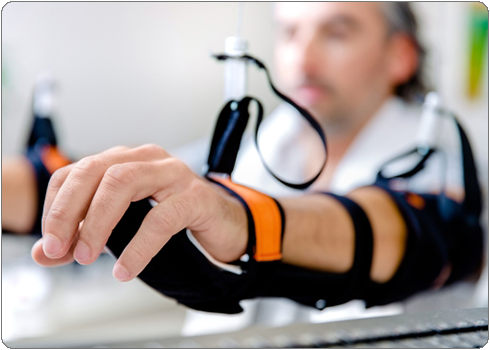
\includegraphics[width=0.5\colwidth]{pics/einleit1}
		\caption{Ein Gerät nach dem Armrobot-Prinzip}
		\label{fig:armrobot}
	\end{figure}

  \end{alertblock}

\end{column}

\separatorcolumn

\begin{column}{\colwidth}  
	
	\begin{alertblock}{Problemstellung}
		\begin{itemize}
			\item Unterstützung der Therapie einer durch Schlaganfall entstandenen Armlähmung mittels eines zu entwickelnden Geräts
			\item Messung der Kontraktion der Armmuskeln und Übertragung an ein Smartphone mit Begleitapp
			\item Motivationsfunktion für Patienten mittels Gamification-Prinzip
			\item Durchführung von Übungen, Minispiel, Erinnerung an Übungen
			\item Ansätze zur Einbindung in eine medizinisch anerkannte Therapiemethode
		\end{itemize}
	\end{alertblock}
  
  \begin{alertblock}{Motivation durch Gamification}
  	\begin{itemize}
  		\item \textbf{Definition:} Verwendung von spieltypischen Mechaniken außerhalb reiner Spiele, mit dem Ziel, das Verhalten von Menschen zu beeinflussen \begin{small}(Breuer)\end{small}
  		\item \textbf{Ziel:} Steigerung der Nutzungsmotivation
  		\item \textbf{Ausnutzung} des menschlichen Spieltriebs:
  		\begin{itemize}
  			\item positive Anreize zur Anregung zu einem bestimmten Verhalten
  			\item negative Anreize wollen vom Nutzer vermieden werden
  		\end{itemize}
  		\item Festlegung klarer Ziele und Regeln, dadurch \textbf{Resultatstransparenz:} Rückmeldung auf Aktionen des Nutzers vorhersehbar
  		\item Nutzer sollte möglichst leicht gewinnen können, aber Spiel darf weder zu einfach noch zu schwierig sein
  		\item \textbf{operante Konditionierung:} Belohnung in variablem Intervall und variabler Menge
  		\item Einsatz \textbf{spieltypischer Mechanismen}:
  		\begin{itemize}
  			\item Punktesystem (Erfahrungspunkte) und Highscores
  			\item Erfolgsanzeige durch Badges oder Fortschrittsanzeigen
  			\item entdeckbare Aufgaben (Quests)
  			\item Epic Meaning (Arbeit an etwas Erstrebenswertem)
  		\end{itemize}
  		\item \textbf{Beispiele:}
  		\begin{itemize}
  			\item Projekt \textsc{The Fun Theory:} Klaviertreppe, Radarfallenlotterie, bunt blinkender Flaschencontainer, tiefster Mülleimer der Welt
  			\item \textsc{Frage-Antwort-Websites:} Quora, Stack Exchange, Stack Overflow
  		\end{itemize}
  	\item motivationssteigernde Wirkung ist wissenschaftlich noch strittig
  	\end{itemize}
  	\begin{figure}[H]
  		\centering
  		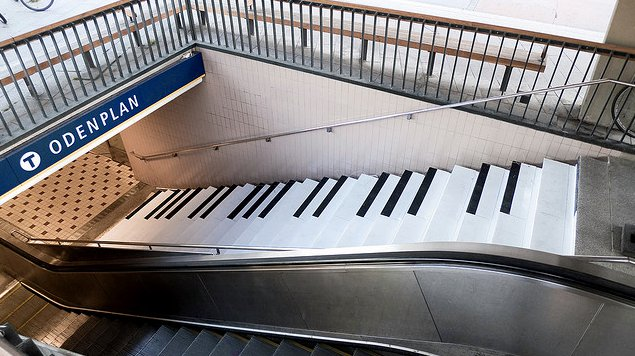
\includegraphics[width=0.5\colwidth]{pics/pianostairs}
  		\caption{Die Klaviertreppe aus dem Projekt \textsc{The Fun Theory}}
  		\label{fig:pianostairs}
  	\end{figure}
  \end{alertblock}

  \begin{alertblock}{Rückkopplung durch Biofeedback}
  	\begin{itemize}
  		\item ständige Veränderung von messbaren Zustandsgrößen bei biologischen Vorgängen und Körperfunktionen
  		\item sind der unmittelbaren Sinneswahrnehmung nicht zugänglich, können jedoch mit elektronischen Hilfsmitteln beobachtbar gemacht werden
  		\item \textbf{Rückkopplung:} Patient kann Kontrolle über die Körperfunktion ausüben
  		\item Messwerte werden visualisiert oder als Töne dargestellt
  		\item tragbare, nichtinvasive Messgeräte unter Verwendung von Analog-Digital-Wandlern und kabelloser Übertragung
  		\item messbare Größen: z.B. Blutwerte, Atem, Hautwiderstand, ...
  	\end{itemize}

    \begin{figure}
      \centering
      \begin{tikzpicture}
        \begin{axis}[
            scale only axis,
            no markers,
            domain=0:2*pi,
            samples=100,
            axis lines=center,
            axis line style={-},
            ticks=none]
          \addplot[red] {sin(deg(x))};
          \addplot[blue] {cos(deg(x))};
        \end{axis}
      \end{tikzpicture}
      \caption{mögliche Visualisierung aufgezeichneter Messwerte}
    \end{figure}

  \end{alertblock}

  \begin{alertblock}{Folgerungen für das Gerät}
  	\begin{itemize}
  		\item Konzeption des Geräts als Unterstützung für Arm-Fähigkeits-Training und Arm-Basis-Training
  		\item Biofeedback durch Messung von Muskelpotentialen per Elektromyografie
  		\item Gamification-System aus:
  		\begin{itemize}
  			\item Erfahrungspunkten
  			\item Badges und Quests
  		\end{itemize}
  	\end{itemize}
  \end{alertblock}

\end{column}

\separatorcolumn
\end{columns}
\end{frame}

\end{document}
